% Översikt över hur roboten ser ut och vad den kan göra

\section{Produkten}

Systemet Gloria är en så kallad \textit{lagerrobot}. Roboten kan autonomt röra sig längs en bana byggd enligt banreglerna som är specificerade i \textit{kravspecifikationen}. Roboten kan endast bära ett paket åt gången och ett paket kan endast sättas ner på en redan tom station . Om roboten upptäcker ett paket den bör plocka upp, stannar den vid stationen och övergår i ett manuellt läge för att låta användaren plocka upp paketet. När användaren signalerar att paketet är greppat övergår roboten i det autonoma läget och fortsätter följa banan till nästa tomma station där den autonomt sätter ner paketet och återigen fortsätter följa banan.

Om roboten inte bär på ett paket avslutar denne sin körning om den kommer till en stoppstation.

\begin{figure}[h!]
	\centering
	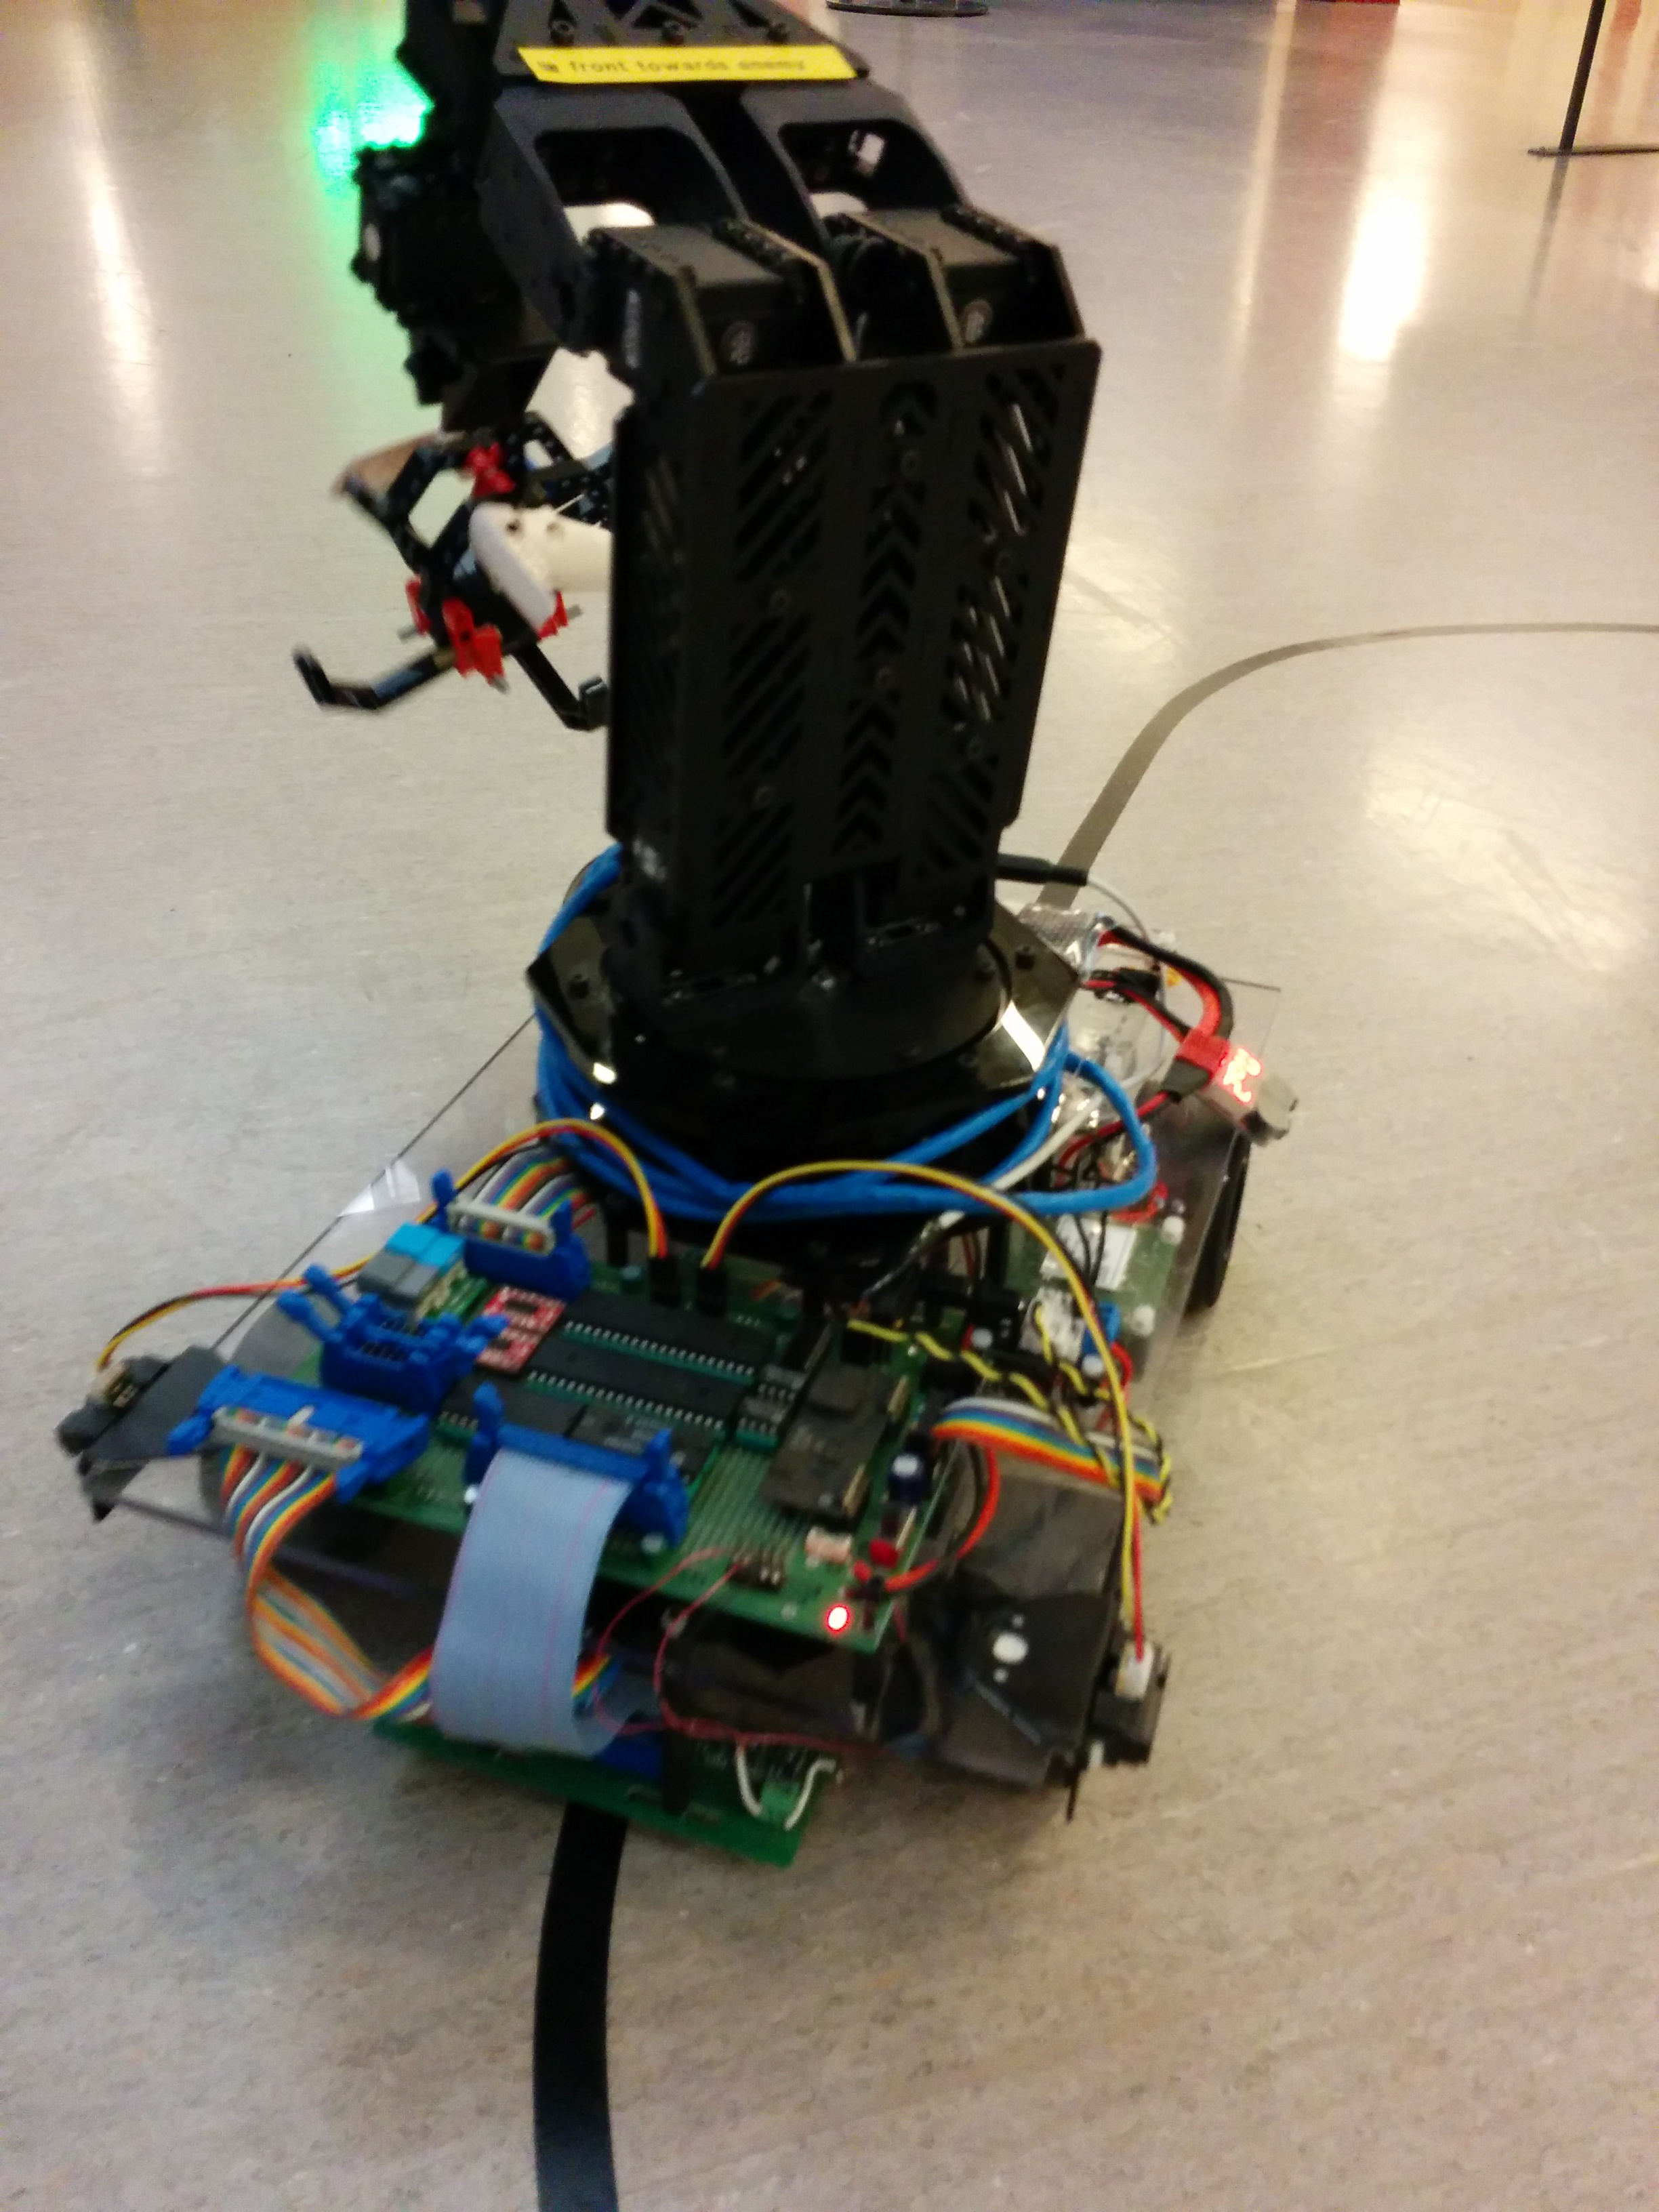
\includegraphics[scale=0.1]{grafik/produkten-gloria.jpg}
	\caption{Systemet i verkligheten} \label{produkten-gloria}
\end{figure}
